% **************************************************************************************************************
% A Classic Thesis Style
% An Homage to The Elements of Typographic Style
%
% Copyright (C) 2015 André Miede http://www.miede.de
%
% If you like the style then I would appreciate a postcard. My address 
% can be found in the file ClassicThesis.pdf. A collection of the 
% postcards I received so far is available online at 
% http://postcards.miede.de
%
% License:
% This program is free software; you can redistribute it and/or modify
% it under the terms of the GNU General Public License as published by
% the Free Software Foundation; either version 2 of the License, or
% (at your option) any later version.
%
% This program is distributed in the hope that it will be useful,
% but WITHOUT ANY WARRANTY; without even the implied warranty of
% MERCHANTABILITY or FITNESS FOR A PARTICULAR PURPOSE.  See the
% GNU General Public License for more details.
%
% You should have received a copy of the GNU General Public License
% along with this program; see the file COPYING.  If not, write to
% the Free Software Foundation, Inc., 59 Temple Place - Suite 330,
% Boston, MA 02111-1307, USA.
%
% **************************************************************************************************************
\RequirePackage{fix-cm} % fix some latex issues see: http://texdoc.net/texmf-dist/doc/latex/base/fixltx2e.pdf
\documentclass[ twoside,openright,titlepage,numbers=noenddot,headinclude,%1headlines,% letterpaper a4paper
                footinclude=true,cleardoublepage=empty,abstractoff, % <--- obsolete, remove (todo)
                BCOR=5mm,paper=a4,fontsize=11pt,%11pt,a4paper,%
                ngerman,american,%
                ]{scrreprt}

%********************************************************************
% Note: Make all your adjustments in here
%*******************************************************
% ****************************************************************************************************
% classicthesis-config.tex 
% formerly known as loadpackages.sty, classicthesis-ldpkg.sty, and classicthesis-preamble.sty 
% Use it at the beginning of your ClassicThesis.tex, or as a LaTeX Preamble 
% in your ClassicThesis.{tex,lyx} with % ****************************************************************************************************
% classicthesis-config.tex 
% formerly known as loadpackages.sty, classicthesis-ldpkg.sty, and classicthesis-preamble.sty 
% Use it at the beginning of your ClassicThesis.tex, or as a LaTeX Preamble 
% in your ClassicThesis.{tex,lyx} with % ****************************************************************************************************
% classicthesis-config.tex 
% formerly known as loadpackages.sty, classicthesis-ldpkg.sty, and classicthesis-preamble.sty 
% Use it at the beginning of your ClassicThesis.tex, or as a LaTeX Preamble 
% in your ClassicThesis.{tex,lyx} with \input{classicthesis-config}
% ****************************************************************************************************  
% If you like the classicthesis, then I would appreciate a postcard. 
% My address can be found in the file ClassicThesis.pdf. A collection 
% of the postcards I received so far is available online at 
% http://postcards.miede.de
% ****************************************************************************************************


% ****************************************************************************************************
% 0. Set the encoding of your files. UTF-8 is the only sensible encoding nowadays. If you can't read
% äöüßáéçèê∂åëæƒÏ€ then change the encoding setting in your editor, not the line below. If your editor
% does not support utf8 use another editor!
% ****************************************************************************************************
\PassOptionsToPackage{utf8}{inputenc}
    \usepackage{inputenc}

% ****************************************************************************************************
% 1. Configure classicthesis for your needs here, e.g., remove "drafting" below 
% in order to deactivate the time-stamp on the pages
% ****************************************************************************************************
\PassOptionsToPackage{eulerchapternumbers,listings,%drafting,%
                      pdfspacing,floatperchapter,%linedheaders,%
                      beramono,dottedtoc,%
                      subfig,eulermath,parts}{classicthesis}                                        
% ********************************************************************
% Available options for classicthesis.sty 
% (see ClassicThesis.pdf for more information):
% drafting
% parts nochapters linedheaders
% eulerchapternumbers beramono eulermath pdfspacing minionprospacing
% tocaligned dottedtoc manychapters
% listings floatperchapter subfig
% ********************************************************************


% ****************************************************************************************************
% 2. Personal data and user ad-hoc commands
% ****************************************************************************************************
\newcommand{\myTitle}{An Online Stream Processor for Timely Dataflow\xspace}
\newcommand{\myName}{Sebastian Wicki\xspace}
\newcommand{\myVersion}{version 0.1\xspace}

% ********************************************************************
% Setup, finetuning, and useful commands
% ********************************************************************
\newcounter{dummy} % necessary for correct hyperlinks (to index, bib, etc.)
\newlength{\abcd} % for ab..z string length calculation
\newcommand{\ie}{i.\,e.}
\newcommand{\Ie}{I.\,e.}
\newcommand{\eg}{e.\,g.}
\newcommand{\Eg}{E.\,g.} 
% ****************************************************************************************************


% ****************************************************************************************************
% 3. Loading some handy packages
% ****************************************************************************************************
% ********************************************************************
% Shut up warnings
% ********************************************************************
\usepackage{silence}
\WarningFilter{scrreprt}{Usage of package `titlesec'}
%\WarningFilter{scrreprt}{Activating an ugly workaround}
\WarningFilter{fixltx2e}{}
\WarningFilter{titlesec}{Non standard sectioning command detected}

% ******************************************************************** 
% Packages with options that might require adjustments
% ******************************************************************** 
%\PassOptionsToPackage{ngerman,american}{babel}   % change this to your language(s)
% Spanish languages need extra options in order to work with this template
%\PassOptionsToPackage{spanish,es-lcroman}{babel}
    \usepackage{babel}                  

\usepackage{hyphenat}
\hyphenation{que-ries data-flow time-stamp time-ly}

\newcommand\TODO[1]{%
\ifthenelse{\equal{#1}{}}%
{\textcolor{Maroon}{\textbf{TODO.}}}%
{{\color{Maroon} \bfseries TODO: #1}}%
}

\usepackage{verbatim}

\usepackage{csquotes}
\PassOptionsToPackage{%
    %backend=biber, %instead of bibtex
    backend=bibtex8,bibencoding=ascii,%
    language=auto,%
    style=numeric-comp,%
    %style=authoryear-comp, % Author 1999, 2010
    %bibstyle=authoryear,dashed=false, % dashed: substitute rep. author with ---
    sorting=nyt, % name, year, title
    maxbibnames=10, % default: 3, et al.
    %backref=true,%
    natbib=true % natbib compatibility mode (\citep and \citet still work)
}{biblatex}
    \usepackage{biblatex}

\PassOptionsToPackage{fleqn}{amsmath}       % math environments and more by the AMS 
    \usepackage{amsmath}

% ******************************************************************** 
% General useful packages
% ******************************************************************** 
\PassOptionsToPackage{T1}{fontenc} % T2A for cyrillics
    \usepackage{fontenc}     
\usepackage{textcomp} % fix warning with missing font shapes
\usepackage{scrhack} % fix warnings when using KOMA with listings package          
\usepackage{xspace} % to get the spacing after macros right  
\usepackage{mparhack} % get marginpar right
\usepackage{fixltx2e} % fixes some LaTeX stuff --> since 2015 in the LaTeX kernel (see below)
%\usepackage[latest]{latexrelease} % will be used once available in more distributions (ISSUE #107)
\PassOptionsToPackage{printonlyused,smaller}{acronym} 
    \usepackage{acronym} % nice macros for handling all acronyms in the thesis
    %\renewcommand{\bflabel}[1]{{#1}\hfill} % fix the list of acronyms --> no longer working
    %\renewcommand*{\acsfont}[1]{\textsc{#1}} 
    \renewcommand*{\aclabelfont}[1]{\acsfont{#1}}
% ****************************************************************************************************


% ****************************************************************************************************
% 4. Setup floats: tables, (sub)figures, and captions
% ****************************************************************************************************
\usepackage{tabularx} % better tables
    \setlength{\extrarowheight}{3pt} % increase table row height
\newcommand{\tableheadline}[1]{\multicolumn{1}{c}{\spacedlowsmallcaps{#1}}}
\newcommand{\myfloatalign}{\centering} % to be used with each float for alignment
\usepackage{caption}
% Thanks to cgnieder and Claus Lahiri
% http://tex.stackexchange.com/questions/69349/spacedlowsmallcaps-in-caption-label
% [REMOVED DUE TO OTHER PROBLEMS, SEE ISSUE #82]    
%\DeclareCaptionLabelFormat{smallcaps}{\bothIfFirst{#1}{~}\MakeTextLowercase{\textsc{#2}}}
%\captionsetup{font=small,labelformat=smallcaps} % format=hang,
\captionsetup{font=small,labelfont=it,format=plain} % format=hang,
\usepackage{subfig}  
% ****************************************************************************************************


% ****************************************************************************************************
% 5. Setup code listings
% ****************************************************************************************************
\usepackage{listings} 
%\lstset{emph={trueIndex,root},emphstyle=\color{BlueViolet}}%\underbar} % for special keywords

% Define Language
\lstdefinelanguage{Rust}
{
  % list of keywords
  morekeywords={
    abstract,alignof,as,become,box,break,const,continue,crate,do,else,enum,
        extern,false,final,fn,for,if,impl,in,let,loop,macro,match,mod,move,mut,
        offsetof,override,priv,proc,pub,pure,ref,return,Self,self,sizeof,
        static,struct,super,trait,true,type,typeof,unsafe,unsized,use,virtual,
        where,while,yield
  },
  otherkeywords={:,\.,|,=,=>,->,\#!,?},
  sensitive, % keywords are not case-sensitive
  morecomment=[l]{//}, % l is for line comment
  morecomment=[s]{/*}{*/}, % s is for start and end delimiter
  morestring=[b]" % defines that strings are enclosed in double quotes
}

\lstset{language=Rust,%C++,
    morekeywords={PassOptionsToPackage,selectlanguage},
    keywordstyle=\color{RoyalBlue},%\bfseries,
    basicstyle=\small\color{darkgray}\ttfamily,
    identifierstyle=\color{Black},
    commentstyle=\color{Green}\ttfamily,
    stringstyle=\color{Maroon}\ttfamily,
    numbers=none,%left,%
    numberstyle=\scriptsize,%\tiny
    stepnumber=5,
    numbersep=8pt,
    showstringspaces=false,
    breaklines=true,
    %frameround=tttt,
    frame=single,
    rulecolor=\color{lstbackground},
    backgroundcolor=\color{lstbackground},
    captionpos=b,
    belowcaptionskip=.75\baselineskip,
    aboveskip=\baselineskip,
} 
% ****************************************************************************************************             


% ****************************************************************************************************
% 6. PDFLaTeX, hyperreferences and citation backreferences
% ****************************************************************************************************
% ********************************************************************
% Using PDFLaTeX
% ********************************************************************
\PassOptionsToPackage{pdftex,hyperfootnotes=false,pdfpagelabels}{hyperref}
    \usepackage{hyperref}  % backref linktocpage pagebackref
\pdfcompresslevel=9
\pdfadjustspacing=1 
\PassOptionsToPackage{pdftex}{graphicx}
    \usepackage{graphicx} 
 

% ********************************************************************
% Hyperreferences
% ********************************************************************
\hypersetup{%
    %draft, % = no hyperlinking at all (useful in b/w printouts)
    colorlinks=true, linktocpage=true, pdfstartpage=3, pdfstartview=FitV,%
    % uncomment the following line if you want to have black links (e.g., for printing)
    %colorlinks=false, linktocpage=false, pdfstartpage=3, pdfstartview=FitV, pdfborder={0 0 0},%
    breaklinks=true, pdfpagemode=UseNone, pageanchor=true, pdfpagemode=UseOutlines,%
    plainpages=false, bookmarksnumbered, bookmarksopen=true, bookmarksopenlevel=1,%
    hypertexnames=true, pdfhighlight=/O,%nesting=true,%frenchlinks,%
    urlcolor=webbrown, linkcolor=RoyalBlue, citecolor=webgreen, %pagecolor=RoyalBlue,%
    %urlcolor=Black, linkcolor=Black, citecolor=Black, %pagecolor=Black,%
    pdftitle={\myTitle},%
    pdfauthor={\textcopyright\ Sebastian Wicki, Systems Group, Department of Computer Science, ETH Zürich},%
    pdfsubject={},%
    pdfkeywords={},%
    pdfcreator={pdfLaTeX},%
    pdfproducer={LaTeX with hyperref and classicthesis}%
}   

% ********************************************************************
% Setup autoreferences
% ********************************************************************
% There are some issues regarding autorefnames
% http://www.ureader.de/msg/136221647.aspx
% http://www.tex.ac.uk/cgi-bin/texfaq2html?label=latexwords
% you have to redefine the makros for the 
% language you use, e.g., american, ngerman
% (as chosen when loading babel/AtBeginDocument)
% ********************************************************************
\makeatletter
\@ifpackageloaded{babel}%
    {%
       \addto\extrasamerican{%
			\renewcommand*{\figureautorefname}{Figure}%
			\renewcommand*{\tableautorefname}{Table}%
			\renewcommand*{\partautorefname}{Part}%
			\renewcommand*{\chapterautorefname}{Chapter}%
			\renewcommand*{\sectionautorefname}{Section}%
			\renewcommand*{\subsectionautorefname}{Section}%
			\renewcommand*{\subsubsectionautorefname}{Section}%     
                }%
       \addto\extrasngerman{% 
			\renewcommand*{\paragraphautorefname}{Absatz}%
			\renewcommand*{\subparagraphautorefname}{Unterabsatz}%
			\renewcommand*{\footnoteautorefname}{Fu\"snote}%
			\renewcommand*{\FancyVerbLineautorefname}{Zeile}%
			\renewcommand*{\theoremautorefname}{Theorem}%
			\renewcommand*{\appendixautorefname}{Anhang}%
			\renewcommand*{\equationautorefname}{Gleichung}%        
			\renewcommand*{\itemautorefname}{Punkt}%
                }%  
            % Fix to getting autorefs for subfigures right (thanks to Belinda Vogt for changing the definition)
            \providecommand{\subfigureautorefname}{\figureautorefname}%             
    }{\relax}
\makeatother


% ****************************************************************************************************
% 7. Last calls before the bar closes
% ****************************************************************************************************
% ********************************************************************
% Development Stuff
% ********************************************************************
%\listfiles
%\PassOptionsToPackage{l2tabu,orthodox,abort}{nag}
%   \usepackage{nag}
%\PassOptionsToPackage{warning, all}{onlyamsmath}
%   \usepackage{onlyamsmath}

% ********************************************************************
% Last, but not least...
% ********************************************************************
\usepackage{classicthesis} 
% ****************************************************************************************************

% ****************************************************************************************************
% 8. Further adjustments (experimental)
% ****************************************************************************************************
% ********************************************************************
% Changing the text area
% ********************************************************************
%\linespread{1.05} % a bit more for Palatino
%\areaset[current]{312pt}{761pt} % 686 (factor 2.2) + 33 head + 42 head \the\footskip
%\setlength{\marginparwidth}{7em}%
%\setlength{\marginparsep}{2em}%

% ********************************************************************
% Using different fonts
% ********************************************************************
%\usepackage[oldstylenums]{kpfonts} % oldstyle notextcomp
%\usepackage[osf]{libertine}
%\usepackage[light,condensed,math]{iwona}
%\renewcommand{\sfdefault}{iwona}
%\usepackage{lmodern} % <-- no osf support :-(
%\usepackage{cfr-lm} % 
%\usepackage[urw-garamond]{mathdesign} <-- no osf support :-(
%\usepackage[default,osfigures]{opensans} % scale=0.95 
%\usepackage[sfdefault]{FiraSans}
% ****************************************************************************************************

% ********************************************************************
% Systems Group title page
% ********************************************************************
\usepackage[masterthesis]{systems-cover/systems-cover}
\covernum{155}
\covertitle{\myTitle}
\coverauthor{\myName}
\coversupervisedby{Dr.\ Desislava Dimitrova \\ Dr.\ John Liagouris \\ Prof.\ Timothy Roscoe}
\coverdate{May 2016 -- November 2016}

% ********************************************************************
% For the Declaration of Originality
% ********************************************************************
\usepackage{pdfpages}

% ****************************************************************************************************  
% If you like the classicthesis, then I would appreciate a postcard. 
% My address can be found in the file ClassicThesis.pdf. A collection 
% of the postcards I received so far is available online at 
% http://postcards.miede.de
% ****************************************************************************************************


% ****************************************************************************************************
% 0. Set the encoding of your files. UTF-8 is the only sensible encoding nowadays. If you can't read
% äöüßáéçèê∂åëæƒÏ€ then change the encoding setting in your editor, not the line below. If your editor
% does not support utf8 use another editor!
% ****************************************************************************************************
\PassOptionsToPackage{utf8}{inputenc}
    \usepackage{inputenc}

% ****************************************************************************************************
% 1. Configure classicthesis for your needs here, e.g., remove "drafting" below 
% in order to deactivate the time-stamp on the pages
% ****************************************************************************************************
\PassOptionsToPackage{eulerchapternumbers,listings,%drafting,%
                      pdfspacing,floatperchapter,%linedheaders,%
                      beramono,dottedtoc,%
                      subfig,eulermath,parts}{classicthesis}                                        
% ********************************************************************
% Available options for classicthesis.sty 
% (see ClassicThesis.pdf for more information):
% drafting
% parts nochapters linedheaders
% eulerchapternumbers beramono eulermath pdfspacing minionprospacing
% tocaligned dottedtoc manychapters
% listings floatperchapter subfig
% ********************************************************************


% ****************************************************************************************************
% 2. Personal data and user ad-hoc commands
% ****************************************************************************************************
\newcommand{\myTitle}{An Online Stream Processor for Timely Dataflow\xspace}
\newcommand{\myName}{Sebastian Wicki\xspace}
\newcommand{\myVersion}{version 0.1\xspace}

% ********************************************************************
% Setup, finetuning, and useful commands
% ********************************************************************
\newcounter{dummy} % necessary for correct hyperlinks (to index, bib, etc.)
\newlength{\abcd} % for ab..z string length calculation
\newcommand{\ie}{i.\,e.}
\newcommand{\Ie}{I.\,e.}
\newcommand{\eg}{e.\,g.}
\newcommand{\Eg}{E.\,g.} 
% ****************************************************************************************************


% ****************************************************************************************************
% 3. Loading some handy packages
% ****************************************************************************************************
% ********************************************************************
% Shut up warnings
% ********************************************************************
\usepackage{silence}
\WarningFilter{scrreprt}{Usage of package `titlesec'}
%\WarningFilter{scrreprt}{Activating an ugly workaround}
\WarningFilter{fixltx2e}{}
\WarningFilter{titlesec}{Non standard sectioning command detected}

% ******************************************************************** 
% Packages with options that might require adjustments
% ******************************************************************** 
%\PassOptionsToPackage{ngerman,american}{babel}   % change this to your language(s)
% Spanish languages need extra options in order to work with this template
%\PassOptionsToPackage{spanish,es-lcroman}{babel}
    \usepackage{babel}                  

\usepackage{hyphenat}
\hyphenation{que-ries data-flow time-stamp time-ly}

\newcommand\TODO[1]{%
\ifthenelse{\equal{#1}{}}%
{\textcolor{Maroon}{\textbf{TODO.}}}%
{{\color{Maroon} \bfseries TODO: #1}}%
}

\usepackage{verbatim}

\usepackage{csquotes}
\PassOptionsToPackage{%
    %backend=biber, %instead of bibtex
    backend=bibtex8,bibencoding=ascii,%
    language=auto,%
    style=numeric-comp,%
    %style=authoryear-comp, % Author 1999, 2010
    %bibstyle=authoryear,dashed=false, % dashed: substitute rep. author with ---
    sorting=nyt, % name, year, title
    maxbibnames=10, % default: 3, et al.
    %backref=true,%
    natbib=true % natbib compatibility mode (\citep and \citet still work)
}{biblatex}
    \usepackage{biblatex}

\PassOptionsToPackage{fleqn}{amsmath}       % math environments and more by the AMS 
    \usepackage{amsmath}

% ******************************************************************** 
% General useful packages
% ******************************************************************** 
\PassOptionsToPackage{T1}{fontenc} % T2A for cyrillics
    \usepackage{fontenc}     
\usepackage{textcomp} % fix warning with missing font shapes
\usepackage{scrhack} % fix warnings when using KOMA with listings package          
\usepackage{xspace} % to get the spacing after macros right  
\usepackage{mparhack} % get marginpar right
\usepackage{fixltx2e} % fixes some LaTeX stuff --> since 2015 in the LaTeX kernel (see below)
%\usepackage[latest]{latexrelease} % will be used once available in more distributions (ISSUE #107)
\PassOptionsToPackage{printonlyused,smaller}{acronym} 
    \usepackage{acronym} % nice macros for handling all acronyms in the thesis
    %\renewcommand{\bflabel}[1]{{#1}\hfill} % fix the list of acronyms --> no longer working
    %\renewcommand*{\acsfont}[1]{\textsc{#1}} 
    \renewcommand*{\aclabelfont}[1]{\acsfont{#1}}
% ****************************************************************************************************


% ****************************************************************************************************
% 4. Setup floats: tables, (sub)figures, and captions
% ****************************************************************************************************
\usepackage{tabularx} % better tables
    \setlength{\extrarowheight}{3pt} % increase table row height
\newcommand{\tableheadline}[1]{\multicolumn{1}{c}{\spacedlowsmallcaps{#1}}}
\newcommand{\myfloatalign}{\centering} % to be used with each float for alignment
\usepackage{caption}
% Thanks to cgnieder and Claus Lahiri
% http://tex.stackexchange.com/questions/69349/spacedlowsmallcaps-in-caption-label
% [REMOVED DUE TO OTHER PROBLEMS, SEE ISSUE #82]    
%\DeclareCaptionLabelFormat{smallcaps}{\bothIfFirst{#1}{~}\MakeTextLowercase{\textsc{#2}}}
%\captionsetup{font=small,labelformat=smallcaps} % format=hang,
\captionsetup{font=small,labelfont=it,format=plain} % format=hang,
\usepackage{subfig}  
% ****************************************************************************************************


% ****************************************************************************************************
% 5. Setup code listings
% ****************************************************************************************************
\usepackage{listings} 
%\lstset{emph={trueIndex,root},emphstyle=\color{BlueViolet}}%\underbar} % for special keywords

% Define Language
\lstdefinelanguage{Rust}
{
  % list of keywords
  morekeywords={
    abstract,alignof,as,become,box,break,const,continue,crate,do,else,enum,
        extern,false,final,fn,for,if,impl,in,let,loop,macro,match,mod,move,mut,
        offsetof,override,priv,proc,pub,pure,ref,return,Self,self,sizeof,
        static,struct,super,trait,true,type,typeof,unsafe,unsized,use,virtual,
        where,while,yield
  },
  otherkeywords={:,\.,|,=,=>,->,\#!,?},
  sensitive, % keywords are not case-sensitive
  morecomment=[l]{//}, % l is for line comment
  morecomment=[s]{/*}{*/}, % s is for start and end delimiter
  morestring=[b]" % defines that strings are enclosed in double quotes
}

\lstset{language=Rust,%C++,
    morekeywords={PassOptionsToPackage,selectlanguage},
    keywordstyle=\color{RoyalBlue},%\bfseries,
    basicstyle=\small\color{darkgray}\ttfamily,
    identifierstyle=\color{Black},
    commentstyle=\color{Green}\ttfamily,
    stringstyle=\color{Maroon}\ttfamily,
    numbers=none,%left,%
    numberstyle=\scriptsize,%\tiny
    stepnumber=5,
    numbersep=8pt,
    showstringspaces=false,
    breaklines=true,
    %frameround=tttt,
    frame=single,
    rulecolor=\color{lstbackground},
    backgroundcolor=\color{lstbackground},
    captionpos=b,
    belowcaptionskip=.75\baselineskip,
    aboveskip=\baselineskip,
} 
% ****************************************************************************************************             


% ****************************************************************************************************
% 6. PDFLaTeX, hyperreferences and citation backreferences
% ****************************************************************************************************
% ********************************************************************
% Using PDFLaTeX
% ********************************************************************
\PassOptionsToPackage{pdftex,hyperfootnotes=false,pdfpagelabels}{hyperref}
    \usepackage{hyperref}  % backref linktocpage pagebackref
\pdfcompresslevel=9
\pdfadjustspacing=1 
\PassOptionsToPackage{pdftex}{graphicx}
    \usepackage{graphicx} 
 

% ********************************************************************
% Hyperreferences
% ********************************************************************
\hypersetup{%
    %draft, % = no hyperlinking at all (useful in b/w printouts)
    colorlinks=true, linktocpage=true, pdfstartpage=3, pdfstartview=FitV,%
    % uncomment the following line if you want to have black links (e.g., for printing)
    %colorlinks=false, linktocpage=false, pdfstartpage=3, pdfstartview=FitV, pdfborder={0 0 0},%
    breaklinks=true, pdfpagemode=UseNone, pageanchor=true, pdfpagemode=UseOutlines,%
    plainpages=false, bookmarksnumbered, bookmarksopen=true, bookmarksopenlevel=1,%
    hypertexnames=true, pdfhighlight=/O,%nesting=true,%frenchlinks,%
    urlcolor=webbrown, linkcolor=RoyalBlue, citecolor=webgreen, %pagecolor=RoyalBlue,%
    %urlcolor=Black, linkcolor=Black, citecolor=Black, %pagecolor=Black,%
    pdftitle={\myTitle},%
    pdfauthor={\textcopyright\ Sebastian Wicki, Systems Group, Department of Computer Science, ETH Zürich},%
    pdfsubject={},%
    pdfkeywords={},%
    pdfcreator={pdfLaTeX},%
    pdfproducer={LaTeX with hyperref and classicthesis}%
}   

% ********************************************************************
% Setup autoreferences
% ********************************************************************
% There are some issues regarding autorefnames
% http://www.ureader.de/msg/136221647.aspx
% http://www.tex.ac.uk/cgi-bin/texfaq2html?label=latexwords
% you have to redefine the makros for the 
% language you use, e.g., american, ngerman
% (as chosen when loading babel/AtBeginDocument)
% ********************************************************************
\makeatletter
\@ifpackageloaded{babel}%
    {%
       \addto\extrasamerican{%
			\renewcommand*{\figureautorefname}{Figure}%
			\renewcommand*{\tableautorefname}{Table}%
			\renewcommand*{\partautorefname}{Part}%
			\renewcommand*{\chapterautorefname}{Chapter}%
			\renewcommand*{\sectionautorefname}{Section}%
			\renewcommand*{\subsectionautorefname}{Section}%
			\renewcommand*{\subsubsectionautorefname}{Section}%     
                }%
       \addto\extrasngerman{% 
			\renewcommand*{\paragraphautorefname}{Absatz}%
			\renewcommand*{\subparagraphautorefname}{Unterabsatz}%
			\renewcommand*{\footnoteautorefname}{Fu\"snote}%
			\renewcommand*{\FancyVerbLineautorefname}{Zeile}%
			\renewcommand*{\theoremautorefname}{Theorem}%
			\renewcommand*{\appendixautorefname}{Anhang}%
			\renewcommand*{\equationautorefname}{Gleichung}%        
			\renewcommand*{\itemautorefname}{Punkt}%
                }%  
            % Fix to getting autorefs for subfigures right (thanks to Belinda Vogt for changing the definition)
            \providecommand{\subfigureautorefname}{\figureautorefname}%             
    }{\relax}
\makeatother


% ****************************************************************************************************
% 7. Last calls before the bar closes
% ****************************************************************************************************
% ********************************************************************
% Development Stuff
% ********************************************************************
%\listfiles
%\PassOptionsToPackage{l2tabu,orthodox,abort}{nag}
%   \usepackage{nag}
%\PassOptionsToPackage{warning, all}{onlyamsmath}
%   \usepackage{onlyamsmath}

% ********************************************************************
% Last, but not least...
% ********************************************************************
\usepackage{classicthesis} 
% ****************************************************************************************************

% ****************************************************************************************************
% 8. Further adjustments (experimental)
% ****************************************************************************************************
% ********************************************************************
% Changing the text area
% ********************************************************************
%\linespread{1.05} % a bit more for Palatino
%\areaset[current]{312pt}{761pt} % 686 (factor 2.2) + 33 head + 42 head \the\footskip
%\setlength{\marginparwidth}{7em}%
%\setlength{\marginparsep}{2em}%

% ********************************************************************
% Using different fonts
% ********************************************************************
%\usepackage[oldstylenums]{kpfonts} % oldstyle notextcomp
%\usepackage[osf]{libertine}
%\usepackage[light,condensed,math]{iwona}
%\renewcommand{\sfdefault}{iwona}
%\usepackage{lmodern} % <-- no osf support :-(
%\usepackage{cfr-lm} % 
%\usepackage[urw-garamond]{mathdesign} <-- no osf support :-(
%\usepackage[default,osfigures]{opensans} % scale=0.95 
%\usepackage[sfdefault]{FiraSans}
% ****************************************************************************************************

% ********************************************************************
% Systems Group title page
% ********************************************************************
\usepackage[masterthesis]{systems-cover/systems-cover}
\covernum{155}
\covertitle{\myTitle}
\coverauthor{\myName}
\coversupervisedby{Dr.\ Desislava Dimitrova \\ Dr.\ John Liagouris \\ Prof.\ Timothy Roscoe}
\coverdate{May 2016 -- November 2016}

% ********************************************************************
% For the Declaration of Originality
% ********************************************************************
\usepackage{pdfpages}

% ****************************************************************************************************  
% If you like the classicthesis, then I would appreciate a postcard. 
% My address can be found in the file ClassicThesis.pdf. A collection 
% of the postcards I received so far is available online at 
% http://postcards.miede.de
% ****************************************************************************************************


% ****************************************************************************************************
% 0. Set the encoding of your files. UTF-8 is the only sensible encoding nowadays. If you can't read
% äöüßáéçèê∂åëæƒÏ€ then change the encoding setting in your editor, not the line below. If your editor
% does not support utf8 use another editor!
% ****************************************************************************************************
\PassOptionsToPackage{utf8}{inputenc}
    \usepackage{inputenc}

% ****************************************************************************************************
% 1. Configure classicthesis for your needs here, e.g., remove "drafting" below 
% in order to deactivate the time-stamp on the pages
% ****************************************************************************************************
\PassOptionsToPackage{eulerchapternumbers,listings,%drafting,%
                      pdfspacing,floatperchapter,%linedheaders,%
                      beramono,dottedtoc,%
                      subfig,eulermath,parts}{classicthesis}                                        
% ********************************************************************
% Available options for classicthesis.sty 
% (see ClassicThesis.pdf for more information):
% drafting
% parts nochapters linedheaders
% eulerchapternumbers beramono eulermath pdfspacing minionprospacing
% tocaligned dottedtoc manychapters
% listings floatperchapter subfig
% ********************************************************************


% ****************************************************************************************************
% 2. Personal data and user ad-hoc commands
% ****************************************************************************************************
\newcommand{\myTitle}{An Online Stream Processor for Timely Dataflow\xspace}
\newcommand{\myName}{Sebastian Wicki\xspace}
\newcommand{\myVersion}{version 0.1\xspace}

% ********************************************************************
% Setup, finetuning, and useful commands
% ********************************************************************
\newcounter{dummy} % necessary for correct hyperlinks (to index, bib, etc.)
\newlength{\abcd} % for ab..z string length calculation
\newcommand{\ie}{i.\,e.}
\newcommand{\Ie}{I.\,e.}
\newcommand{\eg}{e.\,g.}
\newcommand{\Eg}{E.\,g.} 
% ****************************************************************************************************


% ****************************************************************************************************
% 3. Loading some handy packages
% ****************************************************************************************************
% ********************************************************************
% Shut up warnings
% ********************************************************************
\usepackage{silence}
\WarningFilter{scrreprt}{Usage of package `titlesec'}
%\WarningFilter{scrreprt}{Activating an ugly workaround}
\WarningFilter{fixltx2e}{}
\WarningFilter{titlesec}{Non standard sectioning command detected}

% ******************************************************************** 
% Packages with options that might require adjustments
% ******************************************************************** 
%\PassOptionsToPackage{ngerman,american}{babel}   % change this to your language(s)
% Spanish languages need extra options in order to work with this template
%\PassOptionsToPackage{spanish,es-lcroman}{babel}
    \usepackage{babel}                  

\usepackage{hyphenat}
\hyphenation{que-ries data-flow time-stamp time-ly}

\newcommand\TODO[1]{%
\ifthenelse{\equal{#1}{}}%
{\textcolor{Maroon}{\textbf{TODO.}}}%
{{\color{Maroon} \bfseries TODO: #1}}%
}

\usepackage{verbatim}

\usepackage{csquotes}
\PassOptionsToPackage{%
    %backend=biber, %instead of bibtex
    backend=bibtex8,bibencoding=ascii,%
    language=auto,%
    style=numeric-comp,%
    %style=authoryear-comp, % Author 1999, 2010
    %bibstyle=authoryear,dashed=false, % dashed: substitute rep. author with ---
    sorting=nyt, % name, year, title
    maxbibnames=10, % default: 3, et al.
    %backref=true,%
    natbib=true % natbib compatibility mode (\citep and \citet still work)
}{biblatex}
    \usepackage{biblatex}

\PassOptionsToPackage{fleqn}{amsmath}       % math environments and more by the AMS 
    \usepackage{amsmath}

% ******************************************************************** 
% General useful packages
% ******************************************************************** 
\PassOptionsToPackage{T1}{fontenc} % T2A for cyrillics
    \usepackage{fontenc}     
\usepackage{textcomp} % fix warning with missing font shapes
\usepackage{scrhack} % fix warnings when using KOMA with listings package          
\usepackage{xspace} % to get the spacing after macros right  
\usepackage{mparhack} % get marginpar right
\usepackage{fixltx2e} % fixes some LaTeX stuff --> since 2015 in the LaTeX kernel (see below)
%\usepackage[latest]{latexrelease} % will be used once available in more distributions (ISSUE #107)
\PassOptionsToPackage{printonlyused,smaller}{acronym} 
    \usepackage{acronym} % nice macros for handling all acronyms in the thesis
    %\renewcommand{\bflabel}[1]{{#1}\hfill} % fix the list of acronyms --> no longer working
    %\renewcommand*{\acsfont}[1]{\textsc{#1}} 
    \renewcommand*{\aclabelfont}[1]{\acsfont{#1}}
% ****************************************************************************************************


% ****************************************************************************************************
% 4. Setup floats: tables, (sub)figures, and captions
% ****************************************************************************************************
\usepackage{tabularx} % better tables
    \setlength{\extrarowheight}{3pt} % increase table row height
\newcommand{\tableheadline}[1]{\multicolumn{1}{c}{\spacedlowsmallcaps{#1}}}
\newcommand{\myfloatalign}{\centering} % to be used with each float for alignment
\usepackage{caption}
% Thanks to cgnieder and Claus Lahiri
% http://tex.stackexchange.com/questions/69349/spacedlowsmallcaps-in-caption-label
% [REMOVED DUE TO OTHER PROBLEMS, SEE ISSUE #82]    
%\DeclareCaptionLabelFormat{smallcaps}{\bothIfFirst{#1}{~}\MakeTextLowercase{\textsc{#2}}}
%\captionsetup{font=small,labelformat=smallcaps} % format=hang,
\captionsetup{font=small,labelfont=it,format=plain} % format=hang,
\usepackage{subfig}  
% ****************************************************************************************************


% ****************************************************************************************************
% 5. Setup code listings
% ****************************************************************************************************
\usepackage{listings} 
%\lstset{emph={trueIndex,root},emphstyle=\color{BlueViolet}}%\underbar} % for special keywords

% Define Language
\lstdefinelanguage{Rust}
{
  % list of keywords
  morekeywords={
    abstract,alignof,as,become,box,break,const,continue,crate,do,else,enum,
        extern,false,final,fn,for,if,impl,in,let,loop,macro,match,mod,move,mut,
        offsetof,override,priv,proc,pub,pure,ref,return,Self,self,sizeof,
        static,struct,super,trait,true,type,typeof,unsafe,unsized,use,virtual,
        where,while,yield
  },
  otherkeywords={:,\.,|,=,=>,->,\#!,?},
  sensitive, % keywords are not case-sensitive
  morecomment=[l]{//}, % l is for line comment
  morecomment=[s]{/*}{*/}, % s is for start and end delimiter
  morestring=[b]" % defines that strings are enclosed in double quotes
}

\lstset{language=Rust,%C++,
    morekeywords={PassOptionsToPackage,selectlanguage},
    keywordstyle=\color{RoyalBlue},%\bfseries,
    basicstyle=\small\color{darkgray}\ttfamily,
    identifierstyle=\color{Black},
    commentstyle=\color{Green}\ttfamily,
    stringstyle=\color{Maroon}\ttfamily,
    numbers=none,%left,%
    numberstyle=\scriptsize,%\tiny
    stepnumber=5,
    numbersep=8pt,
    showstringspaces=false,
    breaklines=true,
    %frameround=tttt,
    frame=single,
    rulecolor=\color{lstbackground},
    backgroundcolor=\color{lstbackground},
    captionpos=b,
    belowcaptionskip=.75\baselineskip,
    aboveskip=\baselineskip,
} 
% ****************************************************************************************************             


% ****************************************************************************************************
% 6. PDFLaTeX, hyperreferences and citation backreferences
% ****************************************************************************************************
% ********************************************************************
% Using PDFLaTeX
% ********************************************************************
\PassOptionsToPackage{pdftex,hyperfootnotes=false,pdfpagelabels}{hyperref}
    \usepackage{hyperref}  % backref linktocpage pagebackref
\pdfcompresslevel=9
\pdfadjustspacing=1 
\PassOptionsToPackage{pdftex}{graphicx}
    \usepackage{graphicx} 
 

% ********************************************************************
% Hyperreferences
% ********************************************************************
\hypersetup{%
    %draft, % = no hyperlinking at all (useful in b/w printouts)
    colorlinks=true, linktocpage=true, pdfstartpage=3, pdfstartview=FitV,%
    % uncomment the following line if you want to have black links (e.g., for printing)
    %colorlinks=false, linktocpage=false, pdfstartpage=3, pdfstartview=FitV, pdfborder={0 0 0},%
    breaklinks=true, pdfpagemode=UseNone, pageanchor=true, pdfpagemode=UseOutlines,%
    plainpages=false, bookmarksnumbered, bookmarksopen=true, bookmarksopenlevel=1,%
    hypertexnames=true, pdfhighlight=/O,%nesting=true,%frenchlinks,%
    urlcolor=webbrown, linkcolor=RoyalBlue, citecolor=webgreen, %pagecolor=RoyalBlue,%
    %urlcolor=Black, linkcolor=Black, citecolor=Black, %pagecolor=Black,%
    pdftitle={\myTitle},%
    pdfauthor={\textcopyright\ Sebastian Wicki, Systems Group, Department of Computer Science, ETH Zürich},%
    pdfsubject={},%
    pdfkeywords={},%
    pdfcreator={pdfLaTeX},%
    pdfproducer={LaTeX with hyperref and classicthesis}%
}   

% ********************************************************************
% Setup autoreferences
% ********************************************************************
% There are some issues regarding autorefnames
% http://www.ureader.de/msg/136221647.aspx
% http://www.tex.ac.uk/cgi-bin/texfaq2html?label=latexwords
% you have to redefine the makros for the 
% language you use, e.g., american, ngerman
% (as chosen when loading babel/AtBeginDocument)
% ********************************************************************
\makeatletter
\@ifpackageloaded{babel}%
    {%
       \addto\extrasamerican{%
			\renewcommand*{\figureautorefname}{Figure}%
			\renewcommand*{\tableautorefname}{Table}%
			\renewcommand*{\partautorefname}{Part}%
			\renewcommand*{\chapterautorefname}{Chapter}%
			\renewcommand*{\sectionautorefname}{Section}%
			\renewcommand*{\subsectionautorefname}{Section}%
			\renewcommand*{\subsubsectionautorefname}{Section}%     
                }%
       \addto\extrasngerman{% 
			\renewcommand*{\paragraphautorefname}{Absatz}%
			\renewcommand*{\subparagraphautorefname}{Unterabsatz}%
			\renewcommand*{\footnoteautorefname}{Fu\"snote}%
			\renewcommand*{\FancyVerbLineautorefname}{Zeile}%
			\renewcommand*{\theoremautorefname}{Theorem}%
			\renewcommand*{\appendixautorefname}{Anhang}%
			\renewcommand*{\equationautorefname}{Gleichung}%        
			\renewcommand*{\itemautorefname}{Punkt}%
                }%  
            % Fix to getting autorefs for subfigures right (thanks to Belinda Vogt for changing the definition)
            \providecommand{\subfigureautorefname}{\figureautorefname}%             
    }{\relax}
\makeatother


% ****************************************************************************************************
% 7. Last calls before the bar closes
% ****************************************************************************************************
% ********************************************************************
% Development Stuff
% ********************************************************************
%\listfiles
%\PassOptionsToPackage{l2tabu,orthodox,abort}{nag}
%   \usepackage{nag}
%\PassOptionsToPackage{warning, all}{onlyamsmath}
%   \usepackage{onlyamsmath}

% ********************************************************************
% Last, but not least...
% ********************************************************************
\usepackage{classicthesis} 
% ****************************************************************************************************

% ****************************************************************************************************
% 8. Further adjustments (experimental)
% ****************************************************************************************************
% ********************************************************************
% Changing the text area
% ********************************************************************
%\linespread{1.05} % a bit more for Palatino
%\areaset[current]{312pt}{761pt} % 686 (factor 2.2) + 33 head + 42 head \the\footskip
%\setlength{\marginparwidth}{7em}%
%\setlength{\marginparsep}{2em}%

% ********************************************************************
% Using different fonts
% ********************************************************************
%\usepackage[oldstylenums]{kpfonts} % oldstyle notextcomp
%\usepackage[osf]{libertine}
%\usepackage[light,condensed,math]{iwona}
%\renewcommand{\sfdefault}{iwona}
%\usepackage{lmodern} % <-- no osf support :-(
%\usepackage{cfr-lm} % 
%\usepackage[urw-garamond]{mathdesign} <-- no osf support :-(
%\usepackage[default,osfigures]{opensans} % scale=0.95 
%\usepackage[sfdefault]{FiraSans}
% ****************************************************************************************************

% ********************************************************************
% Systems Group title page
% ********************************************************************
\usepackage[masterthesis]{systems-cover/systems-cover}
\covernum{155}
\covertitle{\myTitle}
\coverauthor{\myName}
\coversupervisedby{Dr.\ Desislava Dimitrova \\ Dr.\ John Liagouris \\ Prof.\ Timothy Roscoe}
\coverdate{May 2016 -- November 2016}

% ********************************************************************
% For the Declaration of Originality
% ********************************************************************
\usepackage{pdfpages}


%********************************************************************
% Bibliographies
%*******************************************************
\addbibresource{bibliography.bib}

%********************************************************************
% Hyphenation
%*******************************************************
%\hyphenation{put special hyphenation here}

% ********************************************************************
% GO!GO!GO! MOVE IT!
%*******************************************************
\begin{document}
\frenchspacing
\raggedbottom
\selectlanguage{american} % american ngerman
%\renewcommand*{\bibname}{new name}
%\setbibpreamble{}
\pagenumbering{roman}
\pagestyle{plain}
%********************************************************************
% Frontmatter
%*******************************************************
\cleardoublepage%*******************************************************
% Abstract
%*******************************************************
%\renewcommand{\abstractname}{Abstract}
\pdfbookmark[1]{Abstract}{Abstract}
\begingroup
\let\clearpage\relax
\let\cleardoublepage\relax
\let\cleardoublepage\relax

\chapter*{Abstract}

Processing of unbounded data streams is increasingly important in many
applications. 

In this thesis we present a system for managing Timely Dataflow programs,


We demonstrate 

\endgroup

\cleardoublepage%*******************************************************
% Acknowledgments
%*******************************************************
\pdfbookmark[1]{Acknowledgments}{acknowledgments}

\begingroup
\chapter*{Acknowledgments}

I would like to thank Prof. Timothy Roscoe, not only for providing me with the
opportunity to work on this project, but also for his guidance along the way.

My thanks also goes to my supervisors, Dr. Desislava Dimitrova and Dr. John Liagouris.
This work would not have been possible without their great support and invaluable feedback.

Finally I would like to thank Andrea Lattuada and Zaheer Chothia, as their
initial inputs have gained me a better understanding of the particularities
of Timely Dataflow.

\endgroup

\pagestyle{scrheadings}
\cleardoublepage%*******************************************************
% Table of Contents
%*******************************************************
%\phantomsection
\refstepcounter{dummy}
\pdfbookmark[1]{\contentsname}{tableofcontents}
\setcounter{tocdepth}{2} % <-- 2 includes up to subsections in the ToC
\setcounter{secnumdepth}{3} % <-- 3 numbers up to subsubsections
\manualmark
\markboth{\spacedlowsmallcaps{\contentsname}}{\spacedlowsmallcaps{\contentsname}}
\tableofcontents 
\automark[section]{chapter}
\renewcommand{\chaptermark}[1]{\markboth{\spacedlowsmallcaps{#1}}{\spacedlowsmallcaps{#1}}}
\renewcommand{\sectionmark}[1]{\markright{\thesection\enspace\spacedlowsmallcaps{#1}}}
%*******************************************************
% List of Figures and of the Tables
%*******************************************************
\clearpage

\begingroup 
    \let\clearpage\relax
    \let\cleardoublepage\relax
    \let\cleardoublepage\relax
    %*******************************************************
    % List of Figures
    %*******************************************************    
    %\phantomsection 
    \refstepcounter{dummy}
    %\addcontentsline{toc}{chapter}{\listfigurename}
    \pdfbookmark[1]{\listfigurename}{lof}
    \listoffigures

    \vspace{8ex}

    %*******************************************************
    % List of Tables
    %*******************************************************
    %\phantomsection 
    \refstepcounter{dummy}
    %\addcontentsline{toc}{chapter}{\listtablename}
    \pdfbookmark[1]{\listtablename}{lot}
    \listoftables
        
    \vspace{8ex}
%   \newpage
    
    %*******************************************************
    % List of Listings
    %*******************************************************      
      %\phantomsection 
    \refstepcounter{dummy}
    %\addcontentsline{toc}{chapter}{\lstlistlistingname}
    \pdfbookmark[1]{\lstlistlistingname}{lol}
    \lstlistoflistings 

    \vspace{8ex}

\endgroup

%********************************************************************
% Mainmatter
%*******************************************************
\cleardoublepage\pagenumbering{arabic}
%\setcounter{page}{90}
% use \cleardoublepage here to avoid problems with pdfbookmark
\cleardoublepage
%\part{Thesis}
\chapter{Introduction}\label{ch:introduction}

\section{Motivation}

Many applications today perform real-time monitoring and analytics on
potentially unbounded streams of data. Examples of this include analytics for
web applications and social networks, online processing of sensor data, 
or monitoring and networking in datacenters. As the pool of data sources
in this environment grows larger, and the computations become more complex,
the need for stream management systems and expressive programming models arises.

One such programming model is the \emph{timely dataflow} model, first implemented
and introduced in the Naiad system \cite{naiad}. The timely dataflow model
is a programming model for a wide range of data-parallel algorithms, and it has
been demonstrated to perform well for graph and stream processing, also in the
form of incremental and differential computations \cite{differential}.
Timely dataflow supports stateful operators and iterative computations, while
achieving high throughput and low-latency responses thanks to a decentralized
coordination mechanism for global progress tracking.

In this thesis, we investigate the architecture and implementation of a
management system for running timely dataflow computations. Our work
builds upon the Rust implementation of the timely dataflow model,
simply called \textquote{Timely Dataflow} \cite{timely}.

\section{Contribution}

Being an embeddable library, the provided run-time in the current Rust implementation
only concerns itself with executing and scheduling a single dataflow computation.
It does support the execution in multiple processes distributed across a
static set of machines, launching and deployment of the resulting application
in the cluster however has to be done manually by the user. External inputs are
fed into the dataflow graph by custom client code.

The goal of this thesis is the design and implementation of a system which
provides the following features:

- launching and managing multiple concurrent dataflow programs
- on a dynamic set of machines
- providing mechanisms for dataflow computations to share data stream
- providing mechanisms for system state introspection

\section{Outline}

In chapter \ref{ch:background}, we provide a brief overview of
the Timely Dataflow library, its conceptual model and its implementation. The
system designed and implemented as part of this thesis is introduced and
discussed in detail in the chapters \ref{ch:design} \& \ref{ch:impl}. As our
system allows the dynamic composition of dataflow programs, we evaluate the
overhead of this feature on a realistic workload in chapter \ref{ch:evaluation}.
A survey of related work is presented in chapter \ref{ch:related}, and chapter
\ref{ch:future} closes with future work and conclusions.

\cleardoublepage
\chapter{Timely Dataflow}\label{ch:background}

Timely Dataflow \cite{timely} (\textquote{Timely}) is a Rust library for writing distributed,
cyclic dataflow programs. It is a modular implementation of the \emph{timely dataflow
model} introduced by Naiad \cite{naiad}. 

\section{Computational Model}
\begin{addedbar}
Timely Dataflow is a framework for writing dataflow programs. Dataflow programming
accommodates an execution model which can be represented as a directed graph:
Data flows along edges, while the computational logic in vertices transforms it.
Notable features of Naiad and Timely Dataflow are: Support for structured loops,
stateful vertices and the option for vertices to be notified if given input
rounds of data are completed. \cite{naiad}

In the timely dataflow model, the messages flowing along edges are annotated with
timestamps. Timestamps typically denote input rounds, or within the scope of a
structured loop, the loop iteration count. Timely's progress tracking mechanism requires
timestamps to implement a partial order, such that operators can ask the system
to be notified when there are no more outstanding messages for a given timestamp.
This allows Timely to deliver the actual messages out of order, while 
guaranteeing the operators are informed about the existence of still pending
messages.

Dataflow graphs in Timely are hierarchically structured, allowing
nested subgraphs, called scopes. A scope can define its own clock
domain, where the scope's timestamps are appended to the timestamps of messages
entering from outer scopes. When messages leave a scope again, the inner 
timestamp is stripped. Consequently, Timely implements timestamps
as product types with a defined partial order.

\subsection{Data-Parallelism}

Timely employs a data-parallel approach for scaling the computation. In the
conceptual dataflow graph, the user can specify a data partitioning scheme
on the incident edges of an operator. During execution, the dataflow graph
is instantiated on possibly many worker threads, where each worker maintains
a local copy of the dataflow graph. As data is pushed along the edges of the
conceptual graph, it is sent to the designated worker according to the
partitioning scheme. To put it another way, the data emitted by the vertex
instance on one worker might be pushed to the conceptual successor vertex
hosted on a different worker.

This distribution of work can result in messages being delivered out of
order in regard to their timestamp. This motivates Timely to provide the
progress tracking mechanism described below, which allows operators to
be argue about globally outstanding messages.

\subsection{Progress Tracking}

A key feature of the timely dataflow model is its support for notification
about the advancement of messages in flight, i.e. informing operators about
timestamps for which no more messages will arrive. The set of still observable
timestamps at a certain input edge is derived from the \emph{frontier}. Based 
the partially ordered set of possible timestamps $T$, the frontier (at a given
input and a certain time) is defined as a subset (more precisely, an antichain)
$F = \{t_1, t_2, \dots, t_n \in T \}$
which restricts the set of observable future timestamps
$S_F = \{ t_s \mid \exists t_f \in F: t_s \geq t_f \}$

Operators must ask the system to be notified when the frontier advances. This
is typically done by asking for notification about the progress of messages wit
a given timestamp $t$. The
notification is served when there are no more outstanding messages with
timestamp $t$ or smaller, i.e. there are no more elements in the frontier less
or equal than $t$.

In order not to break notification semantics, operators are only allowed to
produce messages with a timestamp greater or equal $t$ if they hold a
capapility for timestamp $t$. Operators can obtain capabilities for a certain
timestamp either during initialization of the system, or if they receive a
message of the given timestamp.

\section{Implementation}

The implementation of Timely Dataflow consists of two separate Rust libraries,
the \lstinline{time\-ly} crate which implements all functionality related to
dataflow graph construction and progress tracking, while a second library
called \lstinline{time\-ly_\-com\-mu\-ni\-ca\-tion} implements the creation and
initialization of worker threads and provides primitives for communication
between workers and operators. 

\subsection{Programming Interface}

The Timely Dataflow library provides a domain-specific language for expressing
dataflow graphs in Rust. Users create operators (vertices) and connect
them to other operators using stream handles (representing edges).

The Timely library contains implementations for common operators such as
\lstinline{map} or \lstinline{fil\-ter}, but also for more generic combinators
such as \lstinline{un\-ary} or \lstinline{bin\-ary} for implementing custom operators.
Many of the provided operators accept user-provided functions to implement
parts of their logic.

External input is fed to the dataflow computation using input operators. These
provide a handle for external code to push data with assigned timestamps into
the dataflow graph. Operator outputs are represented
by typed \lstinline{Stream} handles, which are used by succeeding operators
to connect the stream to their input ports.

\subsection{Run-time Graph Representation} \label{sec:runtime-graph}

When the executions on a worker starts, Timely assembles the run-time
dataflow graph by executing the user-provided dataflow description. 
When operators are instantiated, they inform the run-time about which
connections they have to other operators and provide and implementation
of the \lstinline{Operate} interface, which is used by Timely for progress
tracking and operator scheduling.

By implementing this interface, operators describe their inputs and
outputs in terms of how much timestamps can advance on the operators internal
paths and what capabilities they initially hold. Via this interface, operators
are also informed about the capabilities and paths of the surrounding operators.

Once construction is complete, the dataflow graph cannot be changed anymore.
Timely requires that every worker hosts exactly the same dataflow graph
structure.

During run-time, Timely's progress tracking will query the operator about its
internal progress, requiring the operator to report how many messages were
consumed and produced on each input or output edge, and also which internal
capabilities it holds on to. Notification about the frontier at the
operator's input edge is also delivered over \lstinline{Operate} interface.

A notable feature of the implementation is that the operator run-time interface
is heavily oriented towards progress tracking. 
As a consequence, this run-time representation of the operator graph does not
allow for introspection of the operator type, the type of data being processed
or the contents of the message queues of a certain operator.

\subsubsection{Operator Scheduling and Execution}

Each Timely worker is responsible for scheduling the operators in its local
dataflow graph instance. Operator scheduling is cooperative and interleaved 
with progress tracking: Operators typically perform work when progress tracking
polls the operator about its internal progress. This means that progress
tracking requests generally result in the execution of any user-provided
operator logic.

Operators are always polled in a round-robin fashion, as the worker does
not know about any of the operators pending messages or other kinds of
internal work to be performed.

\subsubsection{Channel Allocation}

As Timely decouples message delivery from progress notification, there is no
need for a central message channel registry. The allocation of messaging
channels between operators is done bilaterally by the operator themselves,
using specialized endpoint allocators provided by
\lstinline{time\-ly_\-com\-mu\-ni\-ca\-tion}. Messages are typically sent in
batches, where all records within a batch share the same timestamp.

The channel allocator provided by this crate is also used by the workers for
broadcasting and receiving progress messages. Communication between workers
running in different processes communicate over TCP/IP, while workers within
the same process use thread-safe FIFO queues to communicate.
Serialization for communication over the network is done using a serialization
library called Abomonation. It trades high performance serialization and 
deserialization for type safety and requires the same in-memory data layout
at both communication endpoints.

\subsection{Deployment}

Timely allows the computation to be distributed over multiple operating system
processes. These processes host all host the same user-provided number of
worker threads an can be run on different machines. Starting a computation
involves deploying compiled binary executable on all participating machines
and spawning them it in parallel.
The amount of worker threads needs to fixed for a given execution of the
program, as all the workers are fully connected in order to be able to exchange
messages. The addresses of any peer processes is provided programmatically
or alternatively read from a text file.

\end{addedbar}

\cleardoublepage
\chapter{Design}\label{ch:design}

In this chapter we discuss the design of the system. It provides two main
services: Deployment and execution of user-submitted queries, and sharing of
data streams between these queries.

\section{Overall Architecture}

Our system consists of multiple components which are briefly described here.
A dataflow program submitted to run as part of the system is
called a \emph{query}. Following Timely's terminology, the execution of a query
is done by a group of \emph{worker} threads. Each worker manages the scheduling and
progress tracking of the operator in the dataflow graph. 

A query is executed by one or more \emph{executors}. Each executor selected to
execute a query will fetch and invoke the query binary, ultimately spawning the
worker threads. 

All these components are managed by a central process called the \emph{coordinator},
which stores and exposes the system state in the \emph{catalog}. The catalog includes
the list of the available executors, the running queries and what data streams they
are processing.

In addition to managing query execution, the coordinator also provides services
for query composition: Queries can publish the results of their dataflow
computation as \emph{topics}, which in turn other queries can subscribe to.

\begin{table}
    \myfloatalign
  \begin{tabularx}{\textwidth}{>{\scshape}lX} \toprule
    \tableheadline{Component} & \tableheadline{Description} \\ \midrule
    Query & User-submitted Timely program running in the system.\\
    Worker & Thread belonging to a query, driving the computation of its local dataflow graph instance.  \\
    Executor & Process designated to host and spawn queries.\\
    Coordinator & Central process managing all the other components.\\
    Catalog & Data collection storing the system state at the coordinator.\\
    Topic & A named and typed representation of an exposed data stream.\\
    Publisher & Operator for exposing Timely streams by publishing them as a topic.\\
    Subscriber & Operator emitting the data stream published into a given topic.\\
    % submission
    % dataflow graph
    \bottomrule
  \end{tabularx}
  \caption{Terminology of the system}  \label{tab:design-terminology}
\end{table}


\begin{figure}[htb]
  \centering
    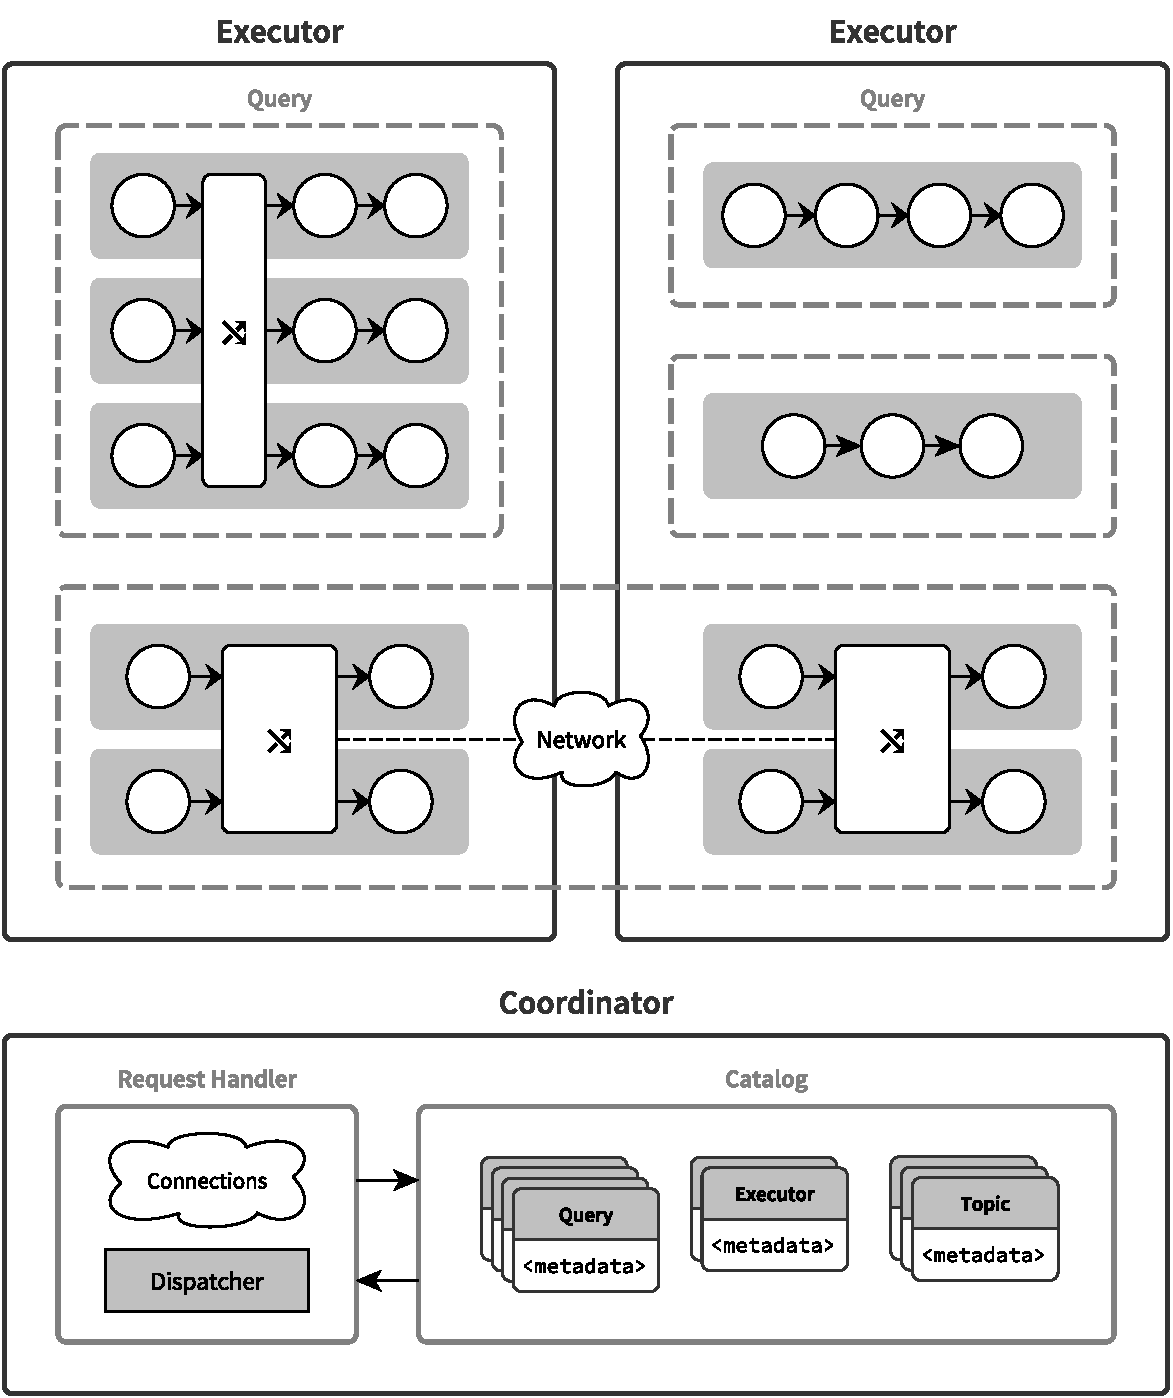
\includegraphics[width=1\textwidth]{figures/components}
  \caption[System architecture.]{ Queries (dashed boxes) consist of one or
  more worker threads (rounded grey boxes) driving the dataflow computation.
  A query might span over multiple executors, make use of the network for message exchanges
  between the workers of a query.\\
  The coordinator maintains a connection to every  executor and every query process.
  The state of the whole system is stored in the catalog.}
  \label{fig:components}
\end{figure}

\clearpage

\section{Queries}

A query is a Timely program managed and executed by our system. Like
standalone Timely Dataflow programs, queries are written in Rust by using the
Timely Dataflow library: The dataflow graph is constructed by connecting
Timely's operators (vertices) to stream objects (edges).

In order for a Timely Dataflow program to become a runnable query on the system,
it needs to link against our query system library. Instead of using Timely's 
initialization functions, a query registers its computational logic with our
\lstinline{timely_query::execute} function.
This function not only performs the initialization of the query according
to submission requests, it also provides additional functionality to interact
with the coordinator. Other than this, there are no restrictions on what the
query program does, it is free to execute arbitrary code.

\begin{lstlisting}[caption={[Example query.]Example query which creates a stream of integers,
filters out all odd numbers and then prints the rest.}]
extern crate timely;
extern crate timely_query;

use timely::dataflow::Scope;
use timely::dataflow::operators::{Filter, Inspect, ToStream};

fn main() {
    timely_query::execute(|root, coordinator| {
        root.scoped::<u32, _, _>(|scope| {
            (0..100).to_stream(scope)
                .filter(|x| x % 2 == 0)
                .inspect(|x| println!("hello {:?}", x));
        });
    }).unwrap();
}
\end{lstlisting}



Timely implements a data-parallel approach for its computation. This is done by
instantiating the dataflow graph on multiple worker threads, where each worker
drives the computation of its local instance, and the data is distributed by
user-provided sharding functions. Workers can be distributed among multiple
machines, where the computation consists of multiple operating system processes
which are communicating with each other over the network. Such an
operating system process might host multiple worker threads.

\begin{figure}[htb]
  \centering
    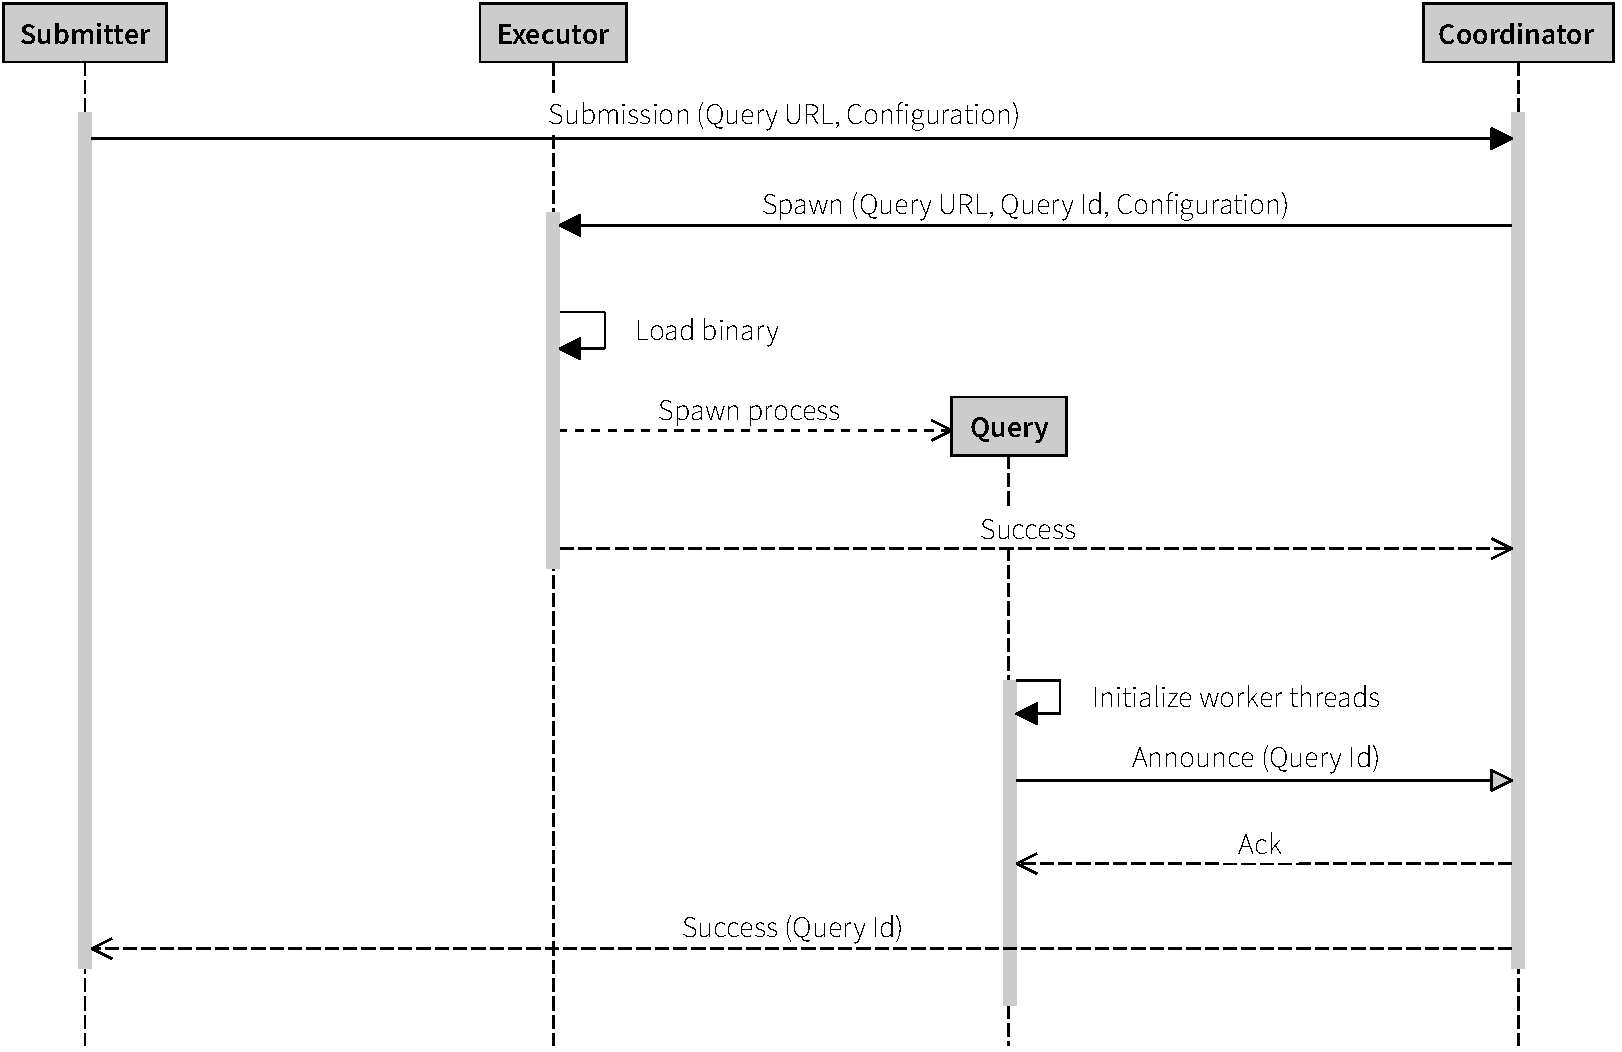
\includegraphics[width=1\textwidth]{figures/spawn_singleprocess}
  \caption[Query submission with single process.]{Submission of a query on a single executor.
  Only once the spawned query announces itself at the coordinator is it considered running.}
  \label{fig:subsingle}
\end{figure}

\section{Executors}

The spawning and direct supervision of query processes is not done by the
coordinator itself, but is offloaded to designated processes called executors.
This choice allows for more flexibility regarding query execution and the
management of available resources. Since executors can be dynamically added
to the system, and with some limitations also be removed again, they provide
a way for adding new machines to the cluster running our system. The catalog
maintains the pool of available executors which are participating in the system.

As a timely program can span over multiple machines, a query might span
over multiple executors. The placement of a query on the available executors
is performed by the coordinator, based on the users request.
We currently implement a naive approach to query placement, where the executors
are chosen randomly if the user does not manually specify a placement. A more
sophisticated scheduling, which for example could include load balancing,
has to be investigated.

Another feature of executors are that they define on how queries and their
worker threads are supposed to be executed. When an executor joins
the system by introducing itself to the coordinator, the executor also informs
the coordinator about the execution format it supports. In the current
implementation, executors only support the execution of queries in the form of
native operating system executables.

When spawning such an executable, the newly spawned query process and the
executor coordinate. The executor supplies the newly created process with the information
it needs in order to participate in the system. This includes the query's own identifier,
the address of the coordinator, the addresses of any peer processes belonging to the 
same query, and the number of worker threads to spawn inside this process.

Executors are also responsible for fetching any query binaries they are supposed
to spawn. When submitting a new query, the submitter has to provide coordinator
with the URL of the binary. This URL is forwarded to participating executors,
which will use it to download the query binary. 

Since executors serve as a provider for computational resources such as machines,
there is typically a one-to-one mapping between executors and the machines they
are running on. This however is not a requirement of the system, the deployment of
executors is left to the user. Similarly, the user is free spawn multiple
processes belonging to the same query on the same executor if they wish to do so.

Since operating system processes can outlive their parent process, executors can
be removed from the system while the queries spawned by the executor are still
running. In this case, the coordinator removes the terminating executor from
the pool, disallowing any future queries to be hosted on the removed executor.

\paragraph{Future Considerations}

The current implementation of executors which run queries in their own separate
process is not the only possible implementation choice.
Alternative implementations could for example host multiple queries
within the same process, by dynamically loading the query's code into an already
running process and run it on a preemptive OS thread. This would allow queries
the interchange of objects without the need for data serialization. Given
the implementation of Timely's operator scheduling, cooperative scheduling
of multiple worker threads within a single operating system thread could also
be implemented for certain queries where its input is managed by the system.
\section{Coordinator}

The purpose of the coordinator is to manage all components of the system. It
provides an interface for users to submit new queries and inspect the current
state of the system. In order to receive commands and report their internal state,
every executor and query process maintains a network connection to the coordinator.

Bookkeeping of the system is done by the coordinator in the catalog. The
catalog is a datastructure which contains all information about the available
executors, the running queries and their workers. 

\subsection{Submission}

A query is submitted to the coordinator as a binary executable. A submission
consists of an URL and format of the query binary, as well as the runtime
configuration for the workers. The runtime configuration specifies the amount
and distribution of the worker threads which will drive the query.

Optionally, a human-readable description of the query,
as well as the command-line arguments to be passed to the executable can be
provided.

When handling a new query submission request, the coordinator will assign a
unique identifier to the incoming query, and then select a
matching number of executors for the query to be spawned on. The selection
of executors is based on the runtime configuration provided by the submission
request.

The coordinator plays an important role when spawning new queries. After
issuing query spawn requests to the executors, it waits for all query processes
to register themselves at the coordinator before they begin their computation.
Only then the query is considered active and the submission request
is reported to be completed.


\section{Sharing Data Streams}

Dataflow programs typically work on streams from external sources. As the same
data source might be of interest for different dataflow computations, it seems
appropriate to also manage input data streams in our system as well. Furthermore,
input streams might not only come from external sources: A dataflow computation
might produce an intermediate or final output stream which could be of interest
for other queries. These assumptions motivate us to extend our system with a
mechanism to allow queries to expose their data streams for consumption by other
queries.

\TODO{Motivation for topic-based pubsub:

- discoverability and type-soundness of topics, type-based reflection hard

- decoupling from producer and consumer (no storing of old data, buffering done by library)

- dynamic adding and removal of topics decoupled from queries lifetime}

We loosely adapted the terminology of publish/subscribe systems: Using the
\emph{publish} operator, a query can expose one of its stream
(an edge in the dataflow graph) to other queries, which in turn then \emph{subscribe}
to it. The list of all published topics is stored at in the catalog.

\subsection{Topics}

A topic has the following properties, which are all stored in the catalog
and can be accessed by other queries.
\begin{description}
\item [Identifier] A unique identifier for the topic instance.
\item [Name] When publishing a stream, the publisher has to assign a name to it.
Queries use this name to refer to topics they want to subscribe to. There might
be only one topic with a certain name at a time, however names can be reused if
topics are unpublished.
\item [Data type] A descriptor of the data type of the stream published in this
topic. Timely's streams are typed channels, therefore so are topics.
\item [Address] An address to which the subscribers connect in order to received
the contents of the published stream.
\end{description}

While every publication and subscription request is disclosed to the coordinator
and the catalog contains a list of all existing topics, the
actual exchange of data happens directly between queries. When a query subscribes
to a topic, it receives the address of the topic's publisher from the coordinator
and directly connects to it.

\subsection{Stream Publisher}

A stream publisher is a Timely operator which exposes a Timely stream as a topic. When
creating it, the query author has to assign a name for the topic under which the
input stream will be published. As with all other Timely operators, the publisher
operator is instantiated on all worker threads. However, the user can choose
whether all worker streams are merged into a single topic before publishing, or
if each worker publishes its own topic. The latter option implicitly exposes
the data sharding strategy of the publishing query, allowing the workers of
the subscribing query to exploit this partition scheme.

\subsubsection{Collection Publisher}

\begin{comment}
This however might be too limiting for some use cases where previously published
data might is essential for a full understanding of the data stream. A simple
solution for this problem would be to buffer the stream at the publisher
and replay it to every incoming subscriber. While simple, this approach
would be wasteful in cases where the data in the buffer becomes stale and
irrelevant to future subscribers. \TODO{this doesn't motivate \emph{unordered}
multisets}
\end{comment}

Normally, publishers are not buffered, meaning subscribers will
not receive any data which was produced before they subscribed to a certain
topic. This is the same as in many other publish/subscribe systems, where
synchronization between publishers and subscribers is decoupled as well. \cite{pubsub}

However, in streams where the contents of the stream describes changes of a certain
state, it is essential for stream consumers to know the state of the source at
the beginning of the stream in order to make sense out of it.

For this reason, we introduce a different kind of publisher which publishes
\emph{collections} instead of streams. A collection is a typed, unordered
multiset maintained by the publisher, possibly representing state it would
like to share with subscribers.

Upon creation, a collection publisher contains an empty collection.
When the publishing query mutates the collection by adding or removing elements,
these changes are propagated to the subscribers. When new subscribers connect
to this publisher, they will initially receive a list of all currently contained
elements. This way, all subscribers eventually maintain the same view of the
data collection.

From the subscribers point of view, a topic published by a collection publisher
is not inherently different from a normal topic: After subscribing, it will
observe a continuous stream of data. The difference is in the data type of the
stream, it will be of tuples of the format $(\texttt{Data}, \delta)$, where
\texttt{Data} is an element that can be stored in the multiset and $\delta$ 
denotes the amount of elements that have been added or removed from the set.
This format
is compatible with the notion of collections in Differential Dataflow, allowing
subscribing queries to further process the collection in a convenient manner.

\subsection{Subscriber}

In order to subscribe to a topic, the subscribing query has to provide the name
of the topic it is interested in. This involves a name lookup which can optionally
be blocking: If a requested topic does not yet exist, the coordinator will add
the subscriber to a wait list. Once a corresponding topic is published under that
name, the coordinator will inform the subscriber about this topic. 

The subscribing query might use different timestamps in its dataflow graph
than the publisher, thus it is the subscribers responsibility to re-add
timestamps to the received stream. 

\subsection{Alternative Approaches}

\subsubsection{Capture \& Replay Operator}

The Timely library also offers the capture and replay operators which serve the
purpose of sharing data between queries. With the capture operator, all timestamp,
data and event records are collected and stored in one dataflow computation,
and can then be replayed in another one.

The implementation of the replay operator requires it to use the same timestamps
as the capture operator, forcing both queries to have a similar structure
in their dataflow graph, as a timestamp received at an operator is defined
by its surrounding scope. Another feature of the capture/replay operator pair
is that they will replay the whole stream from beginning to end, requiring the
capture operator to either buffer its incoming data or wait for the replaying
query to connect to it. 

Both these requirements stem from the fact that the replay operator not only
replays the data stream, but also all progress tracking events, including
notifications. In our system, we opted for a more dynamic approach, where
producing queries are allowed to discard data if there are no consumers, and
where consumers use the streams as inputs for their own computation,
allowing them to assign their own timestamps to the data stream.

It is the user's task to provide a communication channel between capture and 
replay operators. Common channel include Rust's thread-safe FIFO queues or
TCP sockets. In general it can be said the capture/replay operators result
in a more tightly coupled system than publish/subscribe pairs.


\cleardoublepage
%\addtocontents{toc}{\protect\clearpage} % <--- just debug stuff, ignore
%\chapter{Timely Dataflow}\label{ch:background}

Timely Dataflow \cite{timely} (\textquote{Timely}) is a Rust library for writing distributed,
cyclic dataflow programs. It is a modular implementation of the \emph{timely dataflow
model} introduced by Naiad \cite{naiad}. 

\section{Computational Model}
\begin{addedbar}
Timely Dataflow is a framework for writing dataflow programs. Dataflow programming
accommodates an execution model which can be represented as a directed graph:
Data flows along edges, while the computational logic in vertices transforms it.
Notable features of Naiad and Timely Dataflow are: Support for structured loops,
stateful vertices and the option for vertices to be notified if given input
rounds of data are completed. \cite{naiad}

In the timely dataflow model, the messages flowing along edges are annotated with
timestamps. Timestamps typically denote input rounds, or within the scope of a
structured loop, the loop iteration count. Timely's progress tracking mechanism requires
timestamps to implement a partial order, such that operators can ask the system
to be notified when there are no more outstanding messages for a given timestamp.
This allows Timely to deliver the actual messages out of order, while 
guaranteeing the operators are informed about the existence of still pending
messages.

Dataflow graphs in Timely are hierarchically structured, allowing
nested subgraphs, called scopes. A scope can define its own clock
domain, where the scope's timestamps are appended to the timestamps of messages
entering from outer scopes. When messages leave a scope again, the inner 
timestamp is stripped. Consequently, Timely implements timestamps
as product types with a defined partial order.

\subsection{Data-Parallelism}

Timely employs a data-parallel approach for scaling the computation. In the
conceptual dataflow graph, the user can specify a data partitioning scheme
on the incident edges of an operator. During execution, the dataflow graph
is instantiated on possibly many worker threads, where each worker maintains
a local copy of the dataflow graph. As data is pushed along the edges of the
conceptual graph, it is sent to the designated worker according to the
partitioning scheme. To put it another way, the data emitted by the vertex
instance on one worker might be pushed to the conceptual successor vertex
hosted on a different worker.

This distribution of work can result in messages being delivered out of
order in regard to their timestamp. This motivates Timely to provide the
progress tracking mechanism described below, which allows operators to
be argue about globally outstanding messages.

\subsection{Progress Tracking}

A key feature of the timely dataflow model is its support for notification
about the advancement of messages in flight, i.e. informing operators about
timestamps for which no more messages will arrive. The set of still observable
timestamps at a certain input edge is derived from the \emph{frontier}. Based 
the partially ordered set of possible timestamps $T$, the frontier (at a given
input and a certain time) is defined as a subset (more precisely, an antichain)
$F = \{t_1, t_2, \dots, t_n \in T \}$
which restricts the set of observable future timestamps
$S_F = \{ t_s \mid \exists t_f \in F: t_s \geq t_f \}$

Operators must ask the system to be notified when the frontier advances. This
is typically done by asking for notification about the progress of messages wit
a given timestamp $t$. The
notification is served when there are no more outstanding messages with
timestamp $t$ or smaller, i.e. there are no more elements in the frontier less
or equal than $t$.

In order not to break notification semantics, operators are only allowed to
produce messages with a timestamp greater or equal $t$ if they hold a
capapility for timestamp $t$. Operators can obtain capabilities for a certain
timestamp either during initialization of the system, or if they receive a
message of the given timestamp.

\section{Implementation}

The implementation of Timely Dataflow consists of two separate Rust libraries,
the \lstinline{time\-ly} crate which implements all functionality related to
dataflow graph construction and progress tracking, while a second library
called \lstinline{time\-ly_\-com\-mu\-ni\-ca\-tion} implements the creation and
initialization of worker threads and provides primitives for communication
between workers and operators. 

\subsection{Programming Interface}

The Timely Dataflow library provides a domain-specific language for expressing
dataflow graphs in Rust. Users create operators (vertices) and connect
them to other operators using stream handles (representing edges).

The Timely library contains implementations for common operators such as
\lstinline{map} or \lstinline{fil\-ter}, but also for more generic combinators
such as \lstinline{un\-ary} or \lstinline{bin\-ary} for implementing custom operators.
Many of the provided operators accept user-provided functions to implement
parts of their logic.

External input is fed to the dataflow computation using input operators. These
provide a handle for external code to push data with assigned timestamps into
the dataflow graph. Operator outputs are represented
by typed \lstinline{Stream} handles, which are used by succeeding operators
to connect the stream to their input ports.

\subsection{Run-time Graph Representation} \label{sec:runtime-graph}

When the executions on a worker starts, Timely assembles the run-time
dataflow graph by executing the user-provided dataflow description. 
When operators are instantiated, they inform the run-time about which
connections they have to other operators and provide and implementation
of the \lstinline{Operate} interface, which is used by Timely for progress
tracking and operator scheduling.

By implementing this interface, operators describe their inputs and
outputs in terms of how much timestamps can advance on the operators internal
paths and what capabilities they initially hold. Via this interface, operators
are also informed about the capabilities and paths of the surrounding operators.

Once construction is complete, the dataflow graph cannot be changed anymore.
Timely requires that every worker hosts exactly the same dataflow graph
structure.

During run-time, Timely's progress tracking will query the operator about its
internal progress, requiring the operator to report how many messages were
consumed and produced on each input or output edge, and also which internal
capabilities it holds on to. Notification about the frontier at the
operator's input edge is also delivered over \lstinline{Operate} interface.

A notable feature of the implementation is that the operator run-time interface
is heavily oriented towards progress tracking. 
As a consequence, this run-time representation of the operator graph does not
allow for introspection of the operator type, the type of data being processed
or the contents of the message queues of a certain operator.

\subsubsection{Operator Scheduling and Execution}

Each Timely worker is responsible for scheduling the operators in its local
dataflow graph instance. Operator scheduling is cooperative and interleaved 
with progress tracking: Operators typically perform work when progress tracking
polls the operator about its internal progress. This means that progress
tracking requests generally result in the execution of any user-provided
operator logic.

Operators are always polled in a round-robin fashion, as the worker does
not know about any of the operators pending messages or other kinds of
internal work to be performed.

\subsubsection{Channel Allocation}

As Timely decouples message delivery from progress notification, there is no
need for a central message channel registry. The allocation of messaging
channels between operators is done bilaterally by the operator themselves,
using specialized endpoint allocators provided by
\lstinline{time\-ly_\-com\-mu\-ni\-ca\-tion}. Messages are typically sent in
batches, where all records within a batch share the same timestamp.

The channel allocator provided by this crate is also used by the workers for
broadcasting and receiving progress messages. Communication between workers
running in different processes communicate over TCP/IP, while workers within
the same process use thread-safe FIFO queues to communicate.
Serialization for communication over the network is done using a serialization
library called Abomonation. It trades high performance serialization and 
deserialization for type safety and requires the same in-memory data layout
at both communication endpoints.

\subsection{Deployment}

Timely allows the computation to be distributed over multiple operating system
processes. These processes host all host the same user-provided number of
worker threads an can be run on different machines. Starting a computation
involves deploying compiled binary executable on all participating machines
and spawning them it in parallel.
The amount of worker threads needs to fixed for a given execution of the
program, as all the workers are fully connected in order to be able to exchange
messages. The addresses of any peer processes is provided programmatically
or alternatively read from a text file.

\end{addedbar}

%\include{multiToC} % <--- just debug stuff, ignore for your documents
% ********************************************************************
% Backmatter
%*******************************************************
\appendix
%\renewcommand{\thechapter}{\alph{chapter}}
\cleardoublepage
%\part{Appendix}
%********************************************************************
% Appendix
%*******************************************************
% If problems with the headers: get headings in appendix etc. right
%\markboth{\spacedlowsmallcaps{Appendix}}{\spacedlowsmallcaps{Appendix}}
\chapter{Appendix}
Lorem ipsum at nusquam appellantur his, ut eos erant homero
concludaturque. Albucius appellantur deterruisset id eam, vivendum
partiendo dissentiet ei ius. Vis melius facilisis ea, sea id convenire
referrentur, takimata adolescens ex duo. Ei harum argumentum per. Eam
vidit exerci appetere ad, ut vel zzril intellegam interpretaris.

%********************************************************************
% Other Stuff in the Back
%*******************************************************
\cleardoublepage%********************************************************************
% Bibliography
%*******************************************************
% work-around to have small caps also here in the headline
\manualmark
\markboth{\spacedlowsmallcaps{\bibname}}{\spacedlowsmallcaps{\bibname}} % work-around to have small caps also
%\phantomsection 
\refstepcounter{dummy}
\addtocontents{toc}{\protect\vspace{\beforebibskip}} % to have the bib a bit from the rest in the toc
\addcontentsline{toc}{chapter}{\tocEntry{\bibname}}
\label{app:bibliography}
\printbibliography

\pdfbookmark[0]{Declaration of Originality}{declarationoforiginality}
% 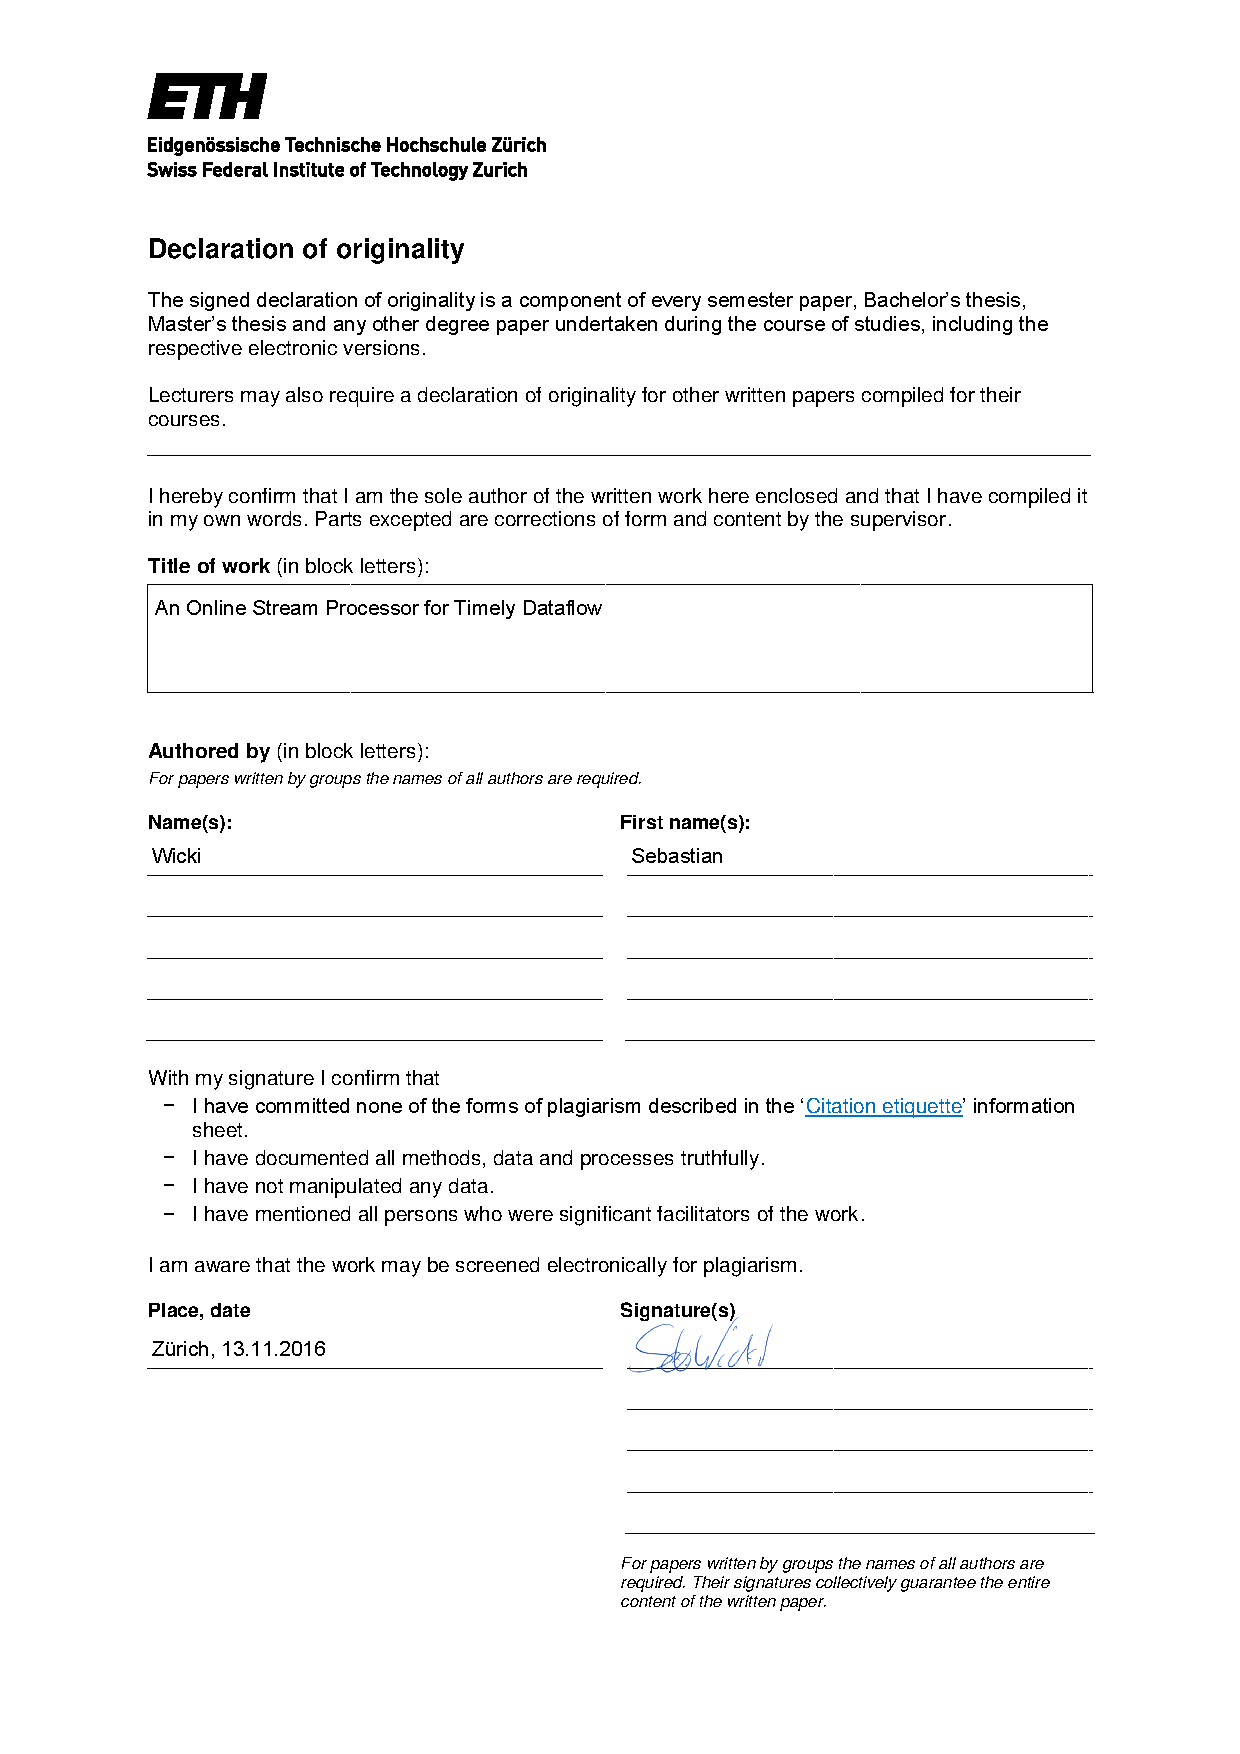
\includepdf[pages={1}]{frontback/declaration-originality.pdf}
% ********************************************************************
% Game Over: Restore, Restart, or Quit?
%*******************************************************
\end{document}
% ********************************************************************
